\mysection{Sacraments}{vulgate-sacraments}

\flavor{\myital{In principio erat Verbum} \\~ \Tilde John 1:1}

  \callout {
    Performing a Sacrament takes Moments; in Combat, invoking a Sacrament is a Combat Action. You only need one hand, and you need to be able to speak. You cannot perform a Sacrament on \mylink{Unhallowed Earth}{occultism-unhallowed-earth}.
}


    The Holy Word of \TheAuthority echoes and reverberates along the branches of Ygg, and flows through the soul of every Mortal being - it is the song of Creation and Order.  Listening to the Word bestows the Grace of \TheAuthority upon you, represented by the d4 \mybold{Grace Die}.


\mysubsection{Grace Die}{vulgate-sacraments-grace}

    The Grace Die is a \UDD{d4} that must be rolled whenever you perform any of the Sacraments. Your Grace Die is returned after you successfully take a \mylink{Bivouac}{combat-resting-bivouac} or longer rest.

    Unless otherwise noted, Sacraments cannot be performed on \mylink{Unhallowed Earth}{occultism-unhallowed-earth} (except Consecrate, of course), and they cannot target the Unhallowed (except for Curse the Unhallowed, of course).  Sacraments do \mybold{not} require a \mylink{Holy Symbol}{liturgies-holy-symbol} to perform; all you need is one free hand and the ability to speak.

  \mysubsection{Bless}{vulgate-sacrament-bless}

   Roll your Grace Die to mark a Mortal Ally or yourself with one of the Signs of the Handmaidens of \TheAuthority. Those so marked can:

\cbreak

\begin{center}
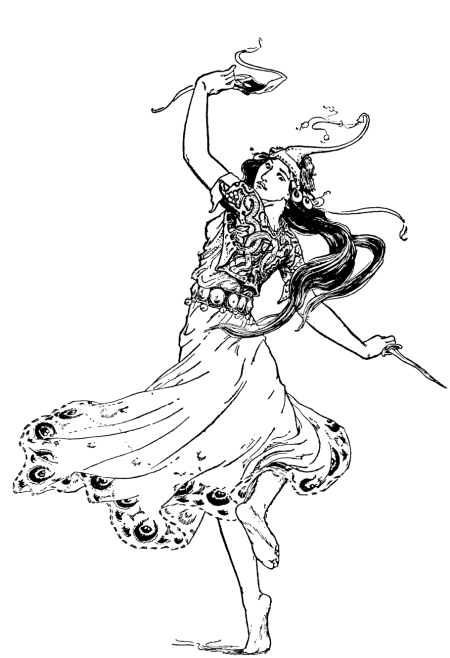
\includegraphics[scale=.45]{vulgate/Sacraments}
\end{center}

    \callout{\footnotesize{
    \mynumlist {
        \item Choose to succeed on their next Save try;
        \item Choose to succeed on their next \\~ \RO or \RB try;
        \item Choose to immediately end a \Duration (on themself);
        \item Choose to succeed on their next \DEATH try.
    }}}

    You must say you're going to use your Blessing \mybold{before you roll your try} i.e. you can't roll, fail, and then decide to use your Blessing.  Once one of the effects of the Blessing is used, it disappears (though the Blessing can be reinvoked).

\newpage

  \mysubsection{Consecrate}{vulgate-sacrament-consecrate}

    You exude a 10 meter diameter circle of \mylink{Hallowed Ground}{miracle-hallowed-ground} around yourself for as long as you maintain Concentration. If you move or are moved from where you are standing, the effect immediately ends. This Sacrament can be performed while you are standing on \mylink{Unhallowed Earth}{occultism-unhallowed-earth}, temporarily canceling its effects (though the ground does not become Hallowed when you do so). Any Unhallowed who do not immediately flee the Consecrated ground are treated as if struck with \mylink{Curse the Unhallowed}{vulgate-sacrament-curse-the-unhallowed}.


  \mysubsection{Curse the Unhallowed}{vulgate-sacrament-curse-the-unhallowed}

   You deal \SUMDICE+1 damage to all Close and Nearby Unhallowed creatures (including Allies, if applicable).


  \mysubsection{Lay on Hands}{vulgate-sacrament-lay-on-hands}

    You can restore up to \SUMDICE+1 points of Mortal Flesh by touch.

\cbreak

  \mysubsection{Loaves and Fishes}{vulgate-sacrament-loaves-fishes}

    You create enough food to feed \SUMDICE+1 people for one meal, along with clean water to fill one mug per person. Mugs, utensils, and condiments are not provided.  Those that participate in the meal do not need to roll \mylink{Provisions}{gear-equipment} for a \mylink{Bivouac}{combat-resting-bivouac}. These Provisions turn to ash in the mouths of the Unhallowed. 

  \mysubsection{Meditation}{vulgate-sacrament-meditation}

    You drop into deep meditation. It needs to be quiet-ish, so you can't do it during Combat. Choose of the following effects and apply it to yourself (only):

\callout{\footnotesize{
    \mybullet {
        \item Restore 1 \UD of any facet of your \mylink{Personality}{adventurer-personality};
        \item Heal \SUMDICE+1 Flesh (up to \MAX); 
        \item Restore \SUMDICE+1 Grit (up to \MAX)
    }
}}


  \mysubsection{Walk on Water}{vulgate-sacrament-walk-water}

   You and up to \SUMDICE+1 Mortal Allies can slowly walk over still water for as long as you maintain Concentration.

